\documentclass[12pt,a4paper]{report}

% Packages
\usepackage[utf8]{inputenc}
\usepackage[T1]{fontenc}
\usepackage{graphicx}
\usepackage{hyperref}
\usepackage{geometry}
\usepackage{booktabs}
\usepackage{float}
\usepackage{caption}
\usepackage{subcaption}
\usepackage{amsmath}
\usepackage{amssymb}
\usepackage{enumitem}
\usepackage{fancyhdr}
\usepackage{titlesec}
\usepackage{xcolor}
\usepackage{listings}
\usepackage{tikz}
\usepackage{array}
\usepackage{multirow}
\usepackage{longtable}
\usepackage{tcolorbox}
\usepackage{setspace}

% TikZ libraries
\usetikzlibrary{shapes.geometric, arrows, positioning, shadows, calc}

% Page geometry
\geometry{margin=1in, headheight=15pt}

% Line spacing
\onehalfspacing

% Colors
\definecolor{primaryblue}{RGB}{26, 115, 232}
\definecolor{darkblue}{RGB}{13, 71, 161}
\definecolor{lightgray}{RGB}{245, 245, 245}
\definecolor{codebg}{RGB}{248, 248, 248}

% Header/Footer
\pagestyle{fancy}
\fancyhf{}
\fancyhead[L]{\leftmark}
\fancyhead[R]{Minor Project Report}
\fancyfoot[C]{\thepage}
\renewcommand{\headrulewidth}{0.4pt}
\renewcommand{\footrulewidth}{0.4pt}

% Hyperref setup
\hypersetup{
    colorlinks=true,
    linkcolor=darkblue,
    filecolor=magenta,
    urlcolor=primaryblue,
    citecolor=darkblue,
    pdftitle={Garbage Classifier for Waste Management},
    pdfauthor={Group 09 - UTD CSVTU Bhilai},
}

% Code listing style
\lstset{
    basicstyle=\ttfamily\small,
    breaklines=true,
    frame=single,
    backgroundcolor=\color{codebg},
    numbers=left,
    numberstyle=\tiny\color{gray},
    keywordstyle=\color{primaryblue}\bfseries,
    commentstyle=\color{gray}\itshape,
    tabsize=4,
    showstringspaces=false
}

% Chapter formatting - each chapter on new page
\titleformat{\chapter}[display]
{\normalfont\huge\bfseries\color{darkblue}}
{\chaptertitlename\ \thechapter}{20pt}{\Huge}
\titlespacing*{\chapter}{0pt}{-20pt}{40pt}

% Section formatting
\titleformat{\section}{\Large\bfseries\color{darkblue}}{\thesection}{1em}{}
\titleformat{\subsection}{\large\bfseries}{\thesubsection}{1em}{}
\titleformat{\subsubsection}{\normalsize\bfseries}{\thesubsubsection}{1em}{}

% Custom box for highlights
\newtcolorbox{highlightbox}[1][]{
    colback=primaryblue!5,
    colframe=primaryblue,
    fonttitle=\bfseries,
    title=#1,
    boxrule=1pt,
    arc=3pt
}

\newtcolorbox{infobox}[1][]{
    colback=lightgray,
    colframe=gray,
    fonttitle=\bfseries,
    title=#1,
    boxrule=0.5pt,
    arc=2pt
}

%=============================================================================
% DOCUMENT BEGINS
%=============================================================================
\begin{document}

%=============================================================================
% TITLE PAGE
%=============================================================================
\begin{titlepage}
    \centering
    \vspace*{1cm}
    
    {\LARGE\textbf{MINOR PROJECT REPORT}\\[0.3cm]}
    {\large On\\[0.5cm]}
    
    {\Huge\textbf{\color{darkblue}Garbage Classifier for\\Waste Management}\\[0.3cm]}
    {\Large\textit{AI-Powered Garbage Segmentation \& Classification System}\\[1cm]}
    
    \includegraphics[width=0.4\textwidth]{docs/screenshots/Main_Application.png}\\[1cm]
    
    {\large\textbf{Submitted By}\\[0.3cm]}
    {\large\textbf{Group Number: 09}\\[0.5cm]}
    
    \begin{tabular}{rl}
        \textbf{1.} & Abhay Singh Sisoodiya \\[3pt]
        \textbf{2.} & Abhinav Anand \\[3pt]
        \textbf{3.} & Aditya Verma \\[3pt]
        \textbf{4.} & Anshul Yadav \\[3pt]
        \textbf{5.} & Aman Banajre \\[3pt]
        \textbf{6.} & Harsh Kumar Chandrakar \\
    \end{tabular}\\[1cm]
    
    {\large\textbf{BTech (Hons.) CSE - Artificial Intelligence}\\
    \textbf{5th Semester}\\[0.5cm]}
    
    \rule{0.6\textwidth}{0.4pt}\\[0.5cm]
    
    {\large University Teaching Department (UTD)\\
    \textbf{Chhattisgarh Swami Vivekanand Technical University (CSVTU)}\\
    Bhilai, Chhattisgarh\\[0.5cm]}
    
    {\large\textbf{December 2025}}
    
\end{titlepage}

%=============================================================================
% TABLE OF CONTENTS
%=============================================================================
\tableofcontents
\listoffigures
\listoftables

%=============================================================================
% CHAPTER 1: ABSTRACT
%=============================================================================
\chapter{Abstract}

\begin{highlightbox}[Project Overview]
This project presents an intelligent \textbf{Garbage Classifier for Waste Management} system that leverages deep learning and computer vision techniques to automatically detect, segment, and classify different types of waste materials.
\end{highlightbox}

\vspace{0.5cm}

Waste management is a critical global issue affecting environmental sustainability, public health, and resource conservation. Improper segregation of garbage contributes to:
\begin{itemize}
    \item Environmental pollution and landfill overflow
    \item Health hazards for sanitation workers
    \item Inefficient recycling and resource recovery
    \item Increased waste processing costs
\end{itemize}

Traditional manual waste sorting is error-prone, labor-intensive, and poses health risks to workers. This project addresses these challenges by developing an AI-powered solution that:

\begin{enumerate}
    \item Uses \textbf{YOLOv8 Instance Segmentation} for precise object detection with pixel-level accuracy
    \item Classifies waste into \textbf{six categories}: biological, cardboard, glass, metal, paper, and plastic
    \item Provides a user-friendly \textbf{Gradio web interface} for real-time predictions
    \item Deploys on \textbf{Hugging Face Spaces} for global accessibility
\end{enumerate}

\begin{infobox}[Key Outcomes]
\begin{itemize}
    \item Trained YOLOv8-Large segmentation model on 481 annotated images
    \item Achieved high accuracy in multi-class garbage classification
    \item Developed production-ready web application
    \item Deployed publicly accessible demo at \url{https://huggingface.co/spaces/Shisodiya/garbage-segmentation}
\end{itemize}
\end{infobox}

%=============================================================================
% CHAPTER 2: INTRODUCTION
%=============================================================================
\chapter{Introduction}

\section{Background}
The rapid increase in urbanization and consumption has led to a significant rise in solid waste generation worldwide. According to the World Bank, global waste generation is projected to increase by 70\% by 2050. Effective waste management is essential for:
\begin{itemize}
    \item Reducing environmental impact
    \item Promoting sustainable development
    \item Supporting circular economy initiatives
    \item Protecting public health
\end{itemize}

\section{Problem Statement}
\begin{highlightbox}[The Challenge]
Improper waste segregation at source is a major bottleneck in the waste management pipeline. Manual sorting is:
\begin{itemize}
    \item \textbf{Time-consuming}: Requires significant human labor
    \item \textbf{Error-prone}: Human fatigue leads to misclassification
    \item \textbf{Hazardous}: Exposes workers to toxic and infectious materials
    \item \textbf{Inconsistent}: Quality varies based on worker expertise
    \item \textbf{Expensive}: High operational costs for large-scale facilities
\end{itemize}
\end{highlightbox}

\section{Proposed Solution}
We propose an AI-based garbage classification system that automates the waste segregation process using computer vision and deep learning. The system architecture includes:

\begin{figure}[H]
    \centering
    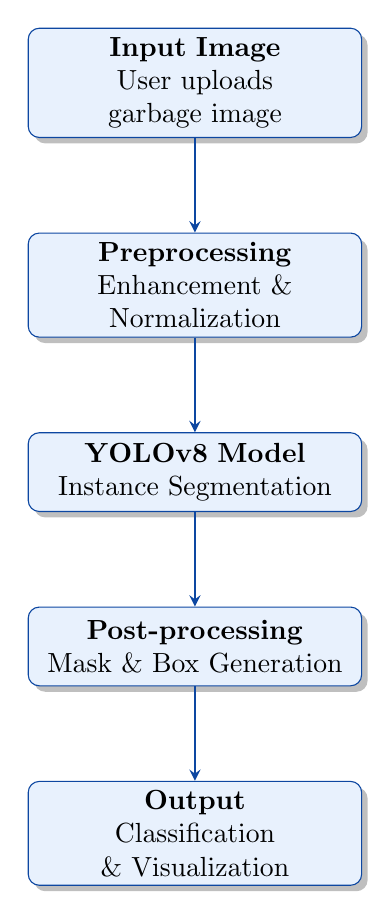
\begin{tikzpicture}[
        node distance=1.2cm,
        box/.style={rectangle, draw=darkblue, fill=primaryblue!10, text width=4cm, minimum height=1cm, align=center, rounded corners, drop shadow},
        arrow/.style={->, >=stealth, thick, darkblue}
    ]
        \node[box] (input) {\textbf{Input Image}\\User uploads garbage image};
        \node[box, below=of input] (preprocess) {\textbf{Preprocessing}\\Enhancement \& Normalization};
        \node[box, below=of preprocess] (model) {\textbf{YOLOv8 Model}\\Instance Segmentation};
        \node[box, below=of model] (postprocess) {\textbf{Post-processing}\\Mask \& Box Generation};
        \node[box, below=of postprocess] (output) {\textbf{Output}\\Classification \& Visualization};
        
        \draw[arrow] (input) -- (preprocess);
        \draw[arrow] (preprocess) -- (model);
        \draw[arrow] (model) -- (postprocess);
        \draw[arrow] (postprocess) -- (output);
    \end{tikzpicture}
    \caption{High-Level System Pipeline}
    \label{fig:pipeline}
\end{figure}

\section{Objectives}
The primary objectives of this project are:

\begin{enumerate}[label=\textbf{O\arabic*.}]
    \item \textbf{Model Development}: Train a YOLOv8-based segmentation model capable of detecting and segmenting garbage objects
    \item \textbf{Multi-class Classification}: Accurately classify waste into 6 categories with high precision and recall
    \item \textbf{User Interface}: Develop an intuitive web interface for easy image upload and result visualization
    \item \textbf{Cloud Deployment}: Deploy the solution on cloud platform for public accessibility
    \item \textbf{Real-time Performance}: Ensure fast inference suitable for practical applications
\end{enumerate}

\section{Scope}
This project focuses on:
\begin{itemize}
    \item Image-based garbage detection (not video or real-time camera)
    \item Six predefined waste categories
    \item Web-based interface (not mobile app)
    \item Cloud deployment on Hugging Face Spaces
\end{itemize}

%=============================================================================
% CHAPTER 3: SYSTEM DESIGN
%=============================================================================
\chapter{System Design and Architecture}

\section{Overall Architecture}
The system follows a modular three-tier architecture separating the presentation layer, application logic, and AI model components.

\begin{figure}[H]
    \centering
    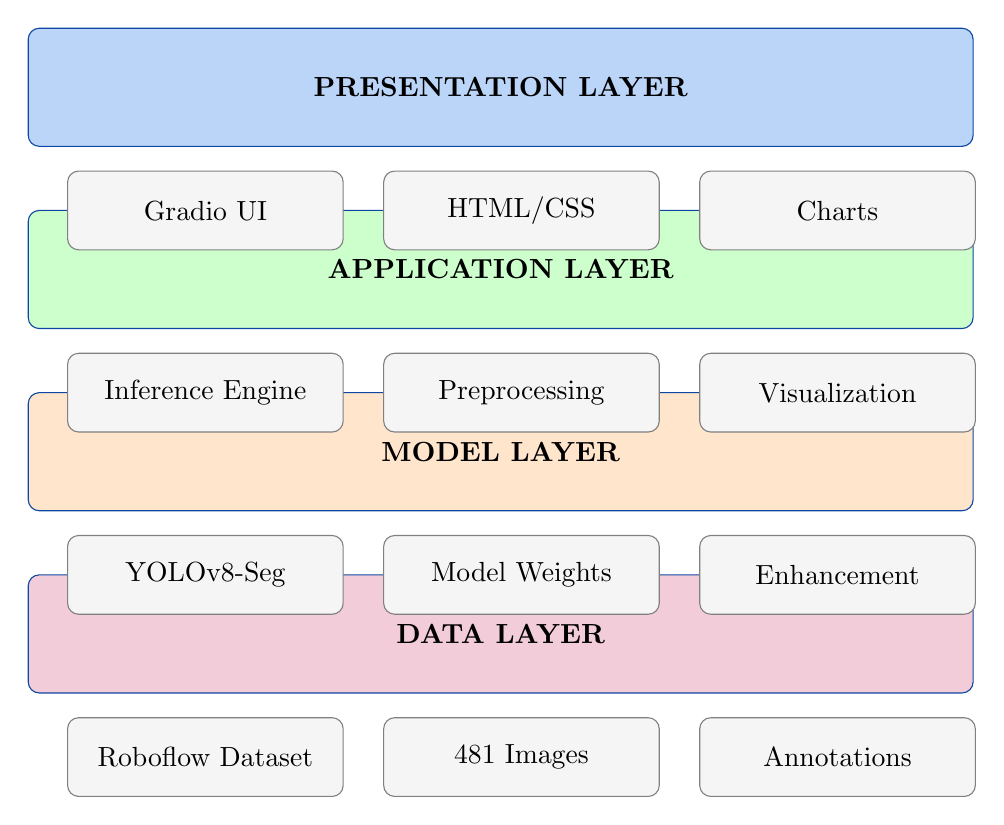
\begin{tikzpicture}[
        node distance=0.8cm,
        layer/.style={rectangle, draw=darkblue, minimum width=12cm, minimum height=1.5cm, align=center, rounded corners},
        component/.style={rectangle, draw=gray, fill=lightgray, minimum width=3.5cm, minimum height=1cm, align=center, rounded corners}
    ]
        % Layers
        \node[layer, fill=primaryblue!30] (presentation) {\textbf{PRESENTATION LAYER}};
        \node[layer, fill=green!20, below=of presentation] (application) {\textbf{APPLICATION LAYER}};
        \node[layer, fill=orange!20, below=of application] (model) {\textbf{MODEL LAYER}};
        \node[layer, fill=purple!20, below=of model] (data) {\textbf{DATA LAYER}};
        
        % Components
        \node[component, below=0.3cm of presentation.south west, anchor=north west, xshift=0.5cm] (gradio) {Gradio UI};
        \node[component, right=0.5cm of gradio] (html) {HTML/CSS};
        \node[component, right=0.5cm of html] (charts) {Charts};
        
        \node[component, below=0.3cm of application.south west, anchor=north west, xshift=0.5cm] (inference) {Inference Engine};
        \node[component, right=0.5cm of inference] (preproc) {Preprocessing};
        \node[component, right=0.5cm of preproc] (viz) {Visualization};
        
        \node[component, below=0.3cm of model.south west, anchor=north west, xshift=0.5cm] (yolo) {YOLOv8-Seg};
        \node[component, right=0.5cm of yolo] (weights) {Model Weights};
        \node[component, right=0.5cm of weights] (enhance) {Enhancement};
        
        \node[component, below=0.3cm of data.south west, anchor=north west, xshift=0.5cm] (dataset) {Roboflow Dataset};
        \node[component, right=0.5cm of dataset] (images) {481 Images};
        \node[component, right=0.5cm of images] (annot) {Annotations};
    \end{tikzpicture}
    \caption{System Architecture Layers}
    \label{fig:architecture}
\end{figure}

\section{Technology Stack}

\begin{table}[H]
    \centering
    \caption{Complete Technology Stack}
    \label{tab:techstack}
    \begin{tabular}{@{}p{3cm}p{3.5cm}p{6cm}@{}}
        \toprule
        \textbf{Category} & \textbf{Technology} & \textbf{Purpose} \\
        \midrule
        \multirow{2}{*}{Deep Learning} & PyTorch 2.0+ & Core deep learning framework \\
        & Ultralytics YOLOv8 & Object detection \& segmentation \\
        \midrule
        \multirow{3}{*}{Computer Vision} & OpenCV & Image processing operations \\
        & PIL/Pillow & Image I/O and manipulation \\
        & NumPy & Numerical computations \\
        \midrule
        \multirow{2}{*}{Web Framework} & Gradio & Interactive ML web interfaces \\
        & HTML/CSS & Custom styling \\
        \midrule
        Visualization & Matplotlib & Charts and graphs generation \\
        \midrule
        \multirow{2}{*}{Deployment} & Hugging Face Spaces & Cloud hosting platform \\
        & Git LFS & Large file storage \\
        \midrule
        Data Management & Roboflow & Dataset hosting \& preprocessing \\
        \bottomrule
    \end{tabular}
\end{table}

\section{YOLOv8 Architecture}
YOLOv8 (You Only Look Once version 8) is a state-of-the-art object detection model developed by Ultralytics. Key architectural features:

\begin{figure}[H]
    \centering
    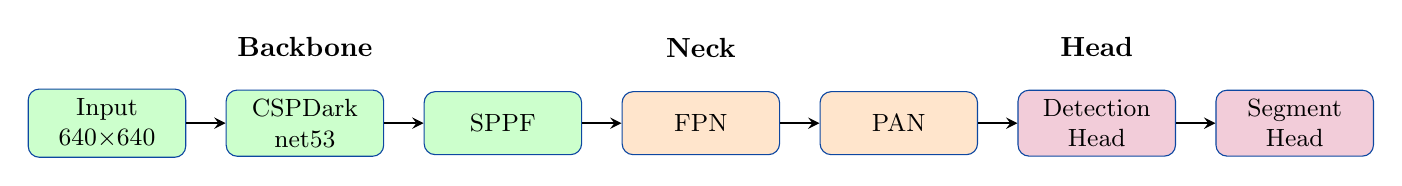
\begin{tikzpicture}[
        node distance=0.5cm,
        block/.style={rectangle, draw=darkblue, fill=primaryblue!10, minimum width=2cm, minimum height=0.8cm, align=center, rounded corners, font=\small},
        arrow/.style={->, >=stealth, thick}
    ]
        % Backbone
        \node[block, fill=green!20] (input) {Input\\640$\times$640};
        \node[block, fill=green!20, right=of input] (csp1) {CSPDark\\net53};
        \node[block, fill=green!20, right=of csp1] (spp) {SPPF};
        
        % Neck
        \node[block, fill=orange!20, right=of spp] (fpn) {FPN};
        \node[block, fill=orange!20, right=of fpn] (pan) {PAN};
        
        % Head
        \node[block, fill=purple!20, right=of pan] (detect) {Detection\\Head};
        \node[block, fill=purple!20, right=of detect] (segment) {Segment\\Head};
        
        % Arrows
        \draw[arrow] (input) -- (csp1);
        \draw[arrow] (csp1) -- (spp);
        \draw[arrow] (spp) -- (fpn);
        \draw[arrow] (fpn) -- (pan);
        \draw[arrow] (pan) -- (detect);
        \draw[arrow] (detect) -- (segment);
        
        % Labels
        \node[above=0.3cm of csp1] {\textbf{Backbone}};
        \node[above=0.3cm of fpn] {\textbf{Neck}};
        \node[above=0.3cm of detect] {\textbf{Head}};
    \end{tikzpicture}
    \caption{YOLOv8 Segmentation Architecture}
    \label{fig:yolo}
\end{figure}

\subsection{Model Variants}
We selected \textbf{YOLOv8-Large (yolov8l-seg)} for optimal balance:

\begin{table}[H]
    \centering
    \caption{YOLOv8 Segmentation Model Variants}
    \label{tab:variants}
    \begin{tabular}{@{}lccccc@{}}
        \toprule
        \textbf{Model} & \textbf{Params (M)} & \textbf{mAP$^{box}$} & \textbf{mAP$^{mask}$} & \textbf{Speed (ms)} \\
        \midrule
        YOLOv8n-seg & 3.4 & 36.7 & 30.5 & 1.21 \\
        YOLOv8s-seg & 11.8 & 44.6 & 36.8 & 1.47 \\
        YOLOv8m-seg & 27.3 & 49.9 & 40.8 & 2.18 \\
        \rowcolor{lightgray}
        \textbf{YOLOv8l-seg} & \textbf{46.0} & \textbf{52.3} & \textbf{42.6} & \textbf{2.79} \\
        YOLOv8x-seg & 71.8 & 53.4 & 43.4 & 4.02 \\
        \bottomrule
    \end{tabular}
\end{table}

%=============================================================================
% CHAPTER 4: DATASET
%=============================================================================
\chapter{Dataset}

\section{Dataset Source}
The dataset was obtained from \textbf{Roboflow Universe}, a community-driven platform for computer vision datasets.

\begin{highlightbox}[Dataset Information]
\begin{tabular}{@{}ll@{}}
    \textbf{Name:} & garbage-segmentation.v2i.yolov8 \\
    \textbf{Source:} & Roboflow Universe \\
    \textbf{License:} & CC BY 4.0 (Creative Commons) \\
    \textbf{Format:} & YOLOv8 Segmentation \\
\end{tabular}
\end{highlightbox}

\section{Dataset Statistics}

\begin{table}[H]
    \centering
    \caption{Dataset Split Statistics}
    \label{tab:dataset_stats}
    \begin{tabular}{@{}lccc@{}}
        \toprule
        \textbf{Property} & \textbf{Training} & \textbf{Validation} & \textbf{Total} \\
        \midrule
        Number of Images & 385 & 96 & 481 \\
        Percentage & 80\% & 20\% & 100\% \\
        Image Size & \multicolumn{3}{c}{640 $\times$ 640 pixels} \\
        Annotation Type & \multicolumn{3}{c}{Polygon Segmentation Masks} \\
        \bottomrule
    \end{tabular}
\end{table}

\section{Class Distribution}
The dataset contains six classes of garbage materials:

\begin{table}[H]
    \centering
    \caption{Garbage Class Descriptions}
    \label{tab:classes}
    \begin{tabular}{@{}clp{8cm}c@{}}
        \toprule
        \textbf{ID} & \textbf{Class} & \textbf{Description} & \textbf{Color} \\
        \midrule
        0 & Biological & Food waste, organic matter, plant materials, biodegradable items & \colorbox{green!40}{Green} \\
        1 & Cardboard & Boxes, packaging materials, corrugated boards, cartons & \colorbox{brown!40}{Brown} \\
        2 & Glass & Bottles, jars, glass containers, broken glass pieces & \colorbox{blue!30}{Blue} \\
        3 & Metal & Aluminum cans, foils, metal containers, tin cans & \colorbox{gray!40}{Gray} \\
        4 & Paper & Documents, newspapers, magazines, paper bags & \colorbox{yellow!40}{Yellow} \\
        5 & Plastic & PET bottles, bags, containers, plastic packaging & \colorbox{red!30}{Red} \\
        \bottomrule
    \end{tabular}
\end{table}

\section{Dataset Visualization}

\begin{figure}[H]
    \centering
    \includegraphics[width=0.9\textwidth]{results/labels.jpg}
    \caption{Dataset Label Distribution: (a) Class instances, (b) Bounding box dimensions, (c) Spatial distribution of objects}
    \label{fig:labels}
\end{figure}

\section{Sample Training Images}

\begin{figure}[H]
    \centering
    \begin{subfigure}[b]{0.45\textwidth}
        \includegraphics[width=\textwidth]{results/train_batch0.jpg}
        \caption{Training Batch 0}
    \end{subfigure}
    \hfill
    \begin{subfigure}[b]{0.45\textwidth}
        \includegraphics[width=\textwidth]{results/train_batch1.jpg}
        \caption{Training Batch 1}
    \end{subfigure}
    \caption{Sample Training Images with Annotations}
    \label{fig:train_samples}
\end{figure}

%=============================================================================
% CHAPTER 5: IMPLEMENTATION
%=============================================================================
\chapter{Implementation}

\section{Development Environment}

\begin{table}[H]
    \centering
    \caption{Development Environment Specifications}
    \label{tab:dev_env}
    \begin{tabular}{@{}ll@{}}
        \toprule
        \textbf{Component} & \textbf{Specification} \\
        \midrule
        Training Platform & Google Colab Pro \\
        GPU & NVIDIA Tesla T4 (16GB VRAM) \\
        Python Version & 3.10+ \\
        PyTorch Version & 2.0+ \\
        Ultralytics Version & 8.0+ \\
        Operating System & Ubuntu 22.04 (Colab) \\
        \bottomrule
    \end{tabular}
\end{table}

\section{Model Training}

\subsection{Training Configuration}
The model was trained with carefully tuned hyperparameters:

\begin{table}[H]
    \centering
    \caption{Training Hyperparameters}
    \label{tab:hyperparams}
    \begin{tabular}{@{}lll@{}}
        \toprule
        \textbf{Parameter} & \textbf{Value} & \textbf{Description} \\
        \midrule
        Base Model & yolov8l-seg.pt & Pre-trained YOLOv8-Large segmentation \\
        Epochs & 200 & Maximum training iterations \\
        Batch Size & 16 & Images per batch \\
        Image Size & 640$\times$640 & Input resolution \\
        Optimizer & AdamW & Advanced Adam with weight decay \\
        Learning Rate & 0.0003 & Initial learning rate \\
        LR Final & 0.01 & Final learning rate (cosine) \\
        Weight Decay & 0.001 & L2 regularization \\
        Patience & 50 & Early stopping patience \\
        IoU Threshold & 0.7 & NMS IoU threshold \\
        \bottomrule
    \end{tabular}
\end{table}

\subsection{Training Command}
\begin{lstlisting}[language=Python, caption=YOLOv8 Training Script]
from ultralytics import YOLO

# Load pre-trained model
model = YOLO('yolov8l-seg.pt')

# Train the model
results = model.train(
    data='data.yaml',
    epochs=200,
    imgsz=640,
    batch=16,
    optimizer='AdamW',
    lr0=0.0003,
    lrf=0.01,
    weight_decay=0.001,
    patience=50,
    cos_lr=True,
    amp=True,  # Mixed precision training
    project='garbage_segmentation',
    name='yolov8l_seg_best'
)
\end{lstlisting}

\subsection{Data Augmentation}
Extensive data augmentation was applied to improve model generalization:

\begin{table}[H]
    \centering
    \caption{Data Augmentation Techniques}
    \label{tab:augmentation}
    \begin{tabular}{@{}llp{6cm}@{}}
        \toprule
        \textbf{Technique} & \textbf{Value} & \textbf{Purpose} \\
        \midrule
        HSV Hue & 0.015 & Color variation for lighting conditions \\
        HSV Saturation & 0.5 & Saturation variation \\
        HSV Value & 0.3 & Brightness variation \\
        Rotation & $\pm$10$^\circ$ & Orientation invariance \\
        Translation & 10\% & Position variation \\
        Scale & 25\% & Size variation \\
        Horizontal Flip & 50\% & Mirror invariance \\
        Mosaic & 50\% & Multi-image composition \\
        MixUp & 5\% & Image blending \\
        Copy-Paste & 30\% & Instance augmentation \\
        RandAugment & Auto & Automated augmentation \\
        \bottomrule
    \end{tabular}
\end{table}

\section{Image Enhancement Module}
To improve accuracy on low-quality images, we implemented a preprocessing module:

\subsection{CLAHE (Contrast Limited Adaptive Histogram Equalization)}
\begin{lstlisting}[language=Python, caption=CLAHE Implementation]
import cv2

def apply_clahe(image):
    """Apply CLAHE for contrast enhancement."""
    lab = cv2.cvtColor(image, cv2.COLOR_RGB2LAB)
    l, a, b = cv2.split(lab)
    
    # Create CLAHE object
    clahe = cv2.createCLAHE(
        clipLimit=2.0, 
        tileGridSize=(8, 8)
    )
    l = clahe.apply(l)
    
    # Merge and convert back
    lab = cv2.merge([l, a, b])
    return cv2.cvtColor(lab, cv2.COLOR_LAB2RGB)
\end{lstlisting}

\subsection{Sharpening Filter}
\begin{lstlisting}[language=Python, caption=Sharpening Filter]
import numpy as np
import cv2

def sharpen_image(image):
    """Apply sharpening filter."""
    kernel = np.array([
        [0, -1, 0],
        [-1, 5, -1],
        [0, -1, 0]
    ], dtype=np.float32)
    return cv2.filter2D(image, -1, kernel)
\end{lstlisting}

\subsection{Auto Brightness Adjustment}
\begin{lstlisting}[language=Python, caption=Auto Brightness Adjustment]
def auto_brightness(image):
    """Automatically adjust brightness."""
    gray = cv2.cvtColor(image, cv2.COLOR_RGB2GRAY)
    mean_brightness = np.mean(gray)
    target = 127
    
    if mean_brightness < 100:  # Too dark
        factor = min(target / (mean_brightness + 1), 2.0)
        return cv2.convertScaleAbs(image, alpha=factor)
    elif mean_brightness > 180:  # Too bright
        factor = target / mean_brightness
        return cv2.convertScaleAbs(image, alpha=factor)
    return image
\end{lstlisting}

\section{Inference Pipeline}

\begin{figure}[H]
    \centering
    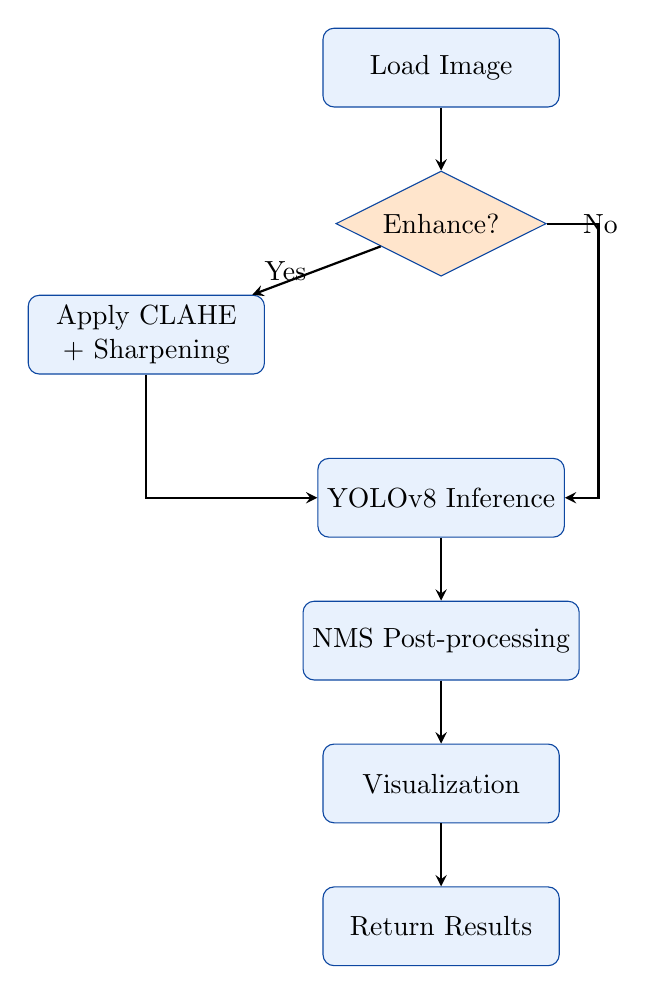
\begin{tikzpicture}[
        node distance=0.8cm,
        block/.style={rectangle, draw=darkblue, fill=primaryblue!10, minimum width=3cm, minimum height=1cm, align=center, rounded corners},
        decision/.style={diamond, draw=darkblue, fill=orange!20, minimum width=2cm, align=center, aspect=2},
        arrow/.style={->, >=stealth, thick}
    ]
        \node[block] (input) {Load Image};
        \node[decision, below=of input] (enhance) {Enhance?};
        \node[block, below left=of enhance, xshift=-1cm] (clahe) {Apply CLAHE\\+ Sharpening};
        \node[block, below=of enhance, yshift=-1.5cm] (model) {YOLOv8 Inference};
        \node[block, below=of model] (nms) {NMS Post-processing};
        \node[block, below=of nms] (visualize) {Visualization};
        \node[block, below=of visualize] (output) {Return Results};
        
        \draw[arrow] (input) -- (enhance);
        \draw[arrow] (enhance) -- node[left] {Yes} (clahe);
        \draw[arrow] (enhance) -- node[right] {No} ++(2,0) |- (model);
        \draw[arrow] (clahe) |- (model);
        \draw[arrow] (model) -- (nms);
        \draw[arrow] (nms) -- (visualize);
        \draw[arrow] (visualize) -- (output);
    \end{tikzpicture}
    \caption{Inference Pipeline Flowchart}
    \label{fig:inference}
\end{figure}

\section{Web Interface Development}
The Gradio interface provides an intuitive user experience:

\begin{lstlisting}[language=Python, caption=Gradio Interface Structure]
import gradio as gr

def create_interface():
    with gr.Blocks(title="Garbage Classifier") as interface:
        # Header
        gr.HTML("<h1>AI Garbage Segmentation System</h1>")
        
        with gr.Row():
            # Input Column
            with gr.Column():
                input_image = gr.Image(label="Upload Image")
                confidence = gr.Slider(0.1, 0.95, value=0.25)
                enhance_toggle = gr.Checkbox(value=True)
                detect_btn = gr.Button("Detect Garbage")
            
            # Output Column
            with gr.Column():
                output_image = gr.Image(label="Results")
                pie_chart = gr.Image(label="Distribution")
                summary = gr.Markdown()
        
        # Event handlers
        detect_btn.click(
            fn=process_image,
            inputs=[input_image, confidence, enhance_toggle],
            outputs=[output_image, pie_chart, summary]
        )
    
    return interface
\end{lstlisting}

%=============================================================================
% CHAPTER 6: RESULTS
%=============================================================================
\chapter{Results and Analysis}

\section{Training Progress}
The model's training metrics over 200 epochs are shown below:

\begin{figure}[H]
    \centering
    \includegraphics[width=\textwidth]{results/results.png}
    \caption{Training and Validation Metrics: Box Loss, Segment Loss, Classification Loss, Precision, Recall, and mAP over epochs}
    \label{fig:results}
\end{figure}

\section{Confusion Matrix Analysis}

\begin{figure}[H]
    \centering
    \begin{subfigure}[b]{0.48\textwidth}
        \centering
        \includegraphics[width=\textwidth]{results/confusion_matrix.png}
        \caption{Absolute Confusion Matrix}
        \label{fig:cm_abs}
    \end{subfigure}
    \hfill
    \begin{subfigure}[b]{0.48\textwidth}
        \centering
        \includegraphics[width=\textwidth]{results/confusion_matrix_normalized.png}
        \caption{Normalized Confusion Matrix}
        \label{fig:cm_norm}
    \end{subfigure}
    \caption{Confusion Matrices showing per-class classification performance}
    \label{fig:confusion}
\end{figure}

\section{Precision-Recall Analysis}

\begin{figure}[H]
    \centering
    \begin{subfigure}[b]{0.48\textwidth}
        \centering
        \includegraphics[width=\textwidth]{results/BoxPR_curve.png}
        \caption{Bounding Box PR Curve}
        \label{fig:box_pr}
    \end{subfigure}
    \hfill
    \begin{subfigure}[b]{0.48\textwidth}
        \centering
        \includegraphics[width=\textwidth]{results/MaskPR_curve.png}
        \caption{Segmentation Mask PR Curve}
        \label{fig:mask_pr}
    \end{subfigure}
    \caption{Precision-Recall Curves for Detection and Segmentation}
    \label{fig:pr_curves}
\end{figure}

\section{F1 Score Analysis}

\begin{figure}[H]
    \centering
    \begin{subfigure}[b]{0.48\textwidth}
        \centering
        \includegraphics[width=\textwidth]{results/BoxF1_curve.png}
        \caption{Box F1-Confidence Curve}
        \label{fig:box_f1}
    \end{subfigure}
    \hfill
    \begin{subfigure}[b]{0.48\textwidth}
        \centering
        \includegraphics[width=\textwidth]{results/MaskF1_curve.png}
        \caption{Mask F1-Confidence Curve}
        \label{fig:mask_f1}
    \end{subfigure}
    \caption{F1 Score vs Confidence Threshold}
    \label{fig:f1_curves}
\end{figure}

\section{Validation Predictions}

\begin{figure}[H]
    \centering
    \begin{subfigure}[b]{0.48\textwidth}
        \centering
        \includegraphics[width=\textwidth]{results/val_batch0_labels.jpg}
        \caption{Ground Truth Labels}
        \label{fig:val_gt}
    \end{subfigure}
    \hfill
    \begin{subfigure}[b]{0.48\textwidth}
        \centering
        \includegraphics[width=\textwidth]{results/val_batch0_pred.jpg}
        \caption{Model Predictions}
        \label{fig:val_pred}
    \end{subfigure}
    \caption{Comparison of Ground Truth vs Model Predictions on Validation Set}
    \label{fig:val_comparison}
\end{figure}

\section{Web Interface Screenshots}

\begin{figure}[H]
    \centering
    \includegraphics[width=0.9\textwidth]{docs/screenshots/Main_Application.png}
    \caption{Gradio Web Interface - Main Application View}
    \label{fig:webapp_main}
\end{figure}

\begin{figure}[H]
    \centering
    \includegraphics[width=0.9\textwidth]{docs/screenshots/Model_detect.png}
    \caption{Detection Results with Segmentation Masks and Class Distribution}
    \label{fig:webapp_detection}
\end{figure}

%=============================================================================
% CHAPTER 7: DEPLOYMENT
%=============================================================================
\chapter{Deployment}

\section{Platform Selection}
We chose \textbf{Hugging Face Spaces} for deployment due to:

\begin{itemize}
    \item \textbf{Free Hosting}: No cost for academic and open-source projects
    \item \textbf{Gradio Integration}: Native support for Gradio applications
    \item \textbf{Git LFS Support}: Handles large model files (92MB+)
    \item \textbf{Public URL}: Accessible worldwide without installation
    \item \textbf{Community}: Large ML community for visibility
\end{itemize}

\section{Deployment Configuration}

\begin{lstlisting}[caption=Hugging Face Space Configuration (README.md)]
---
title: Garbage Classifier for Waste Management
emoji: trash_can:
colorFrom: green
colorTo: blue
sdk: gradio
sdk_version: 3.50.2
app_file: app.py
pinned: false
license: mit
---
\end{lstlisting}

\section{Live Demo}

\begin{highlightbox}[Access the Application]
\centering
\Large\textbf{\url{https://huggingface.co/spaces/Shisodiya/garbage-segmentation}}
\end{highlightbox}

\section{Deployment Files}

\begin{table}[H]
    \centering
    \caption{Files Deployed to Hugging Face Spaces}
    \label{tab:deploy_files}
    \begin{tabular}{@{}llr@{}}
        \toprule
        \textbf{File/Directory} & \textbf{Description} & \textbf{Size} \\
        \midrule
        app.py & Entry point script & 1 KB \\
        requirements.txt & Python dependencies & 1 KB \\
        README.md & Space configuration & 1 KB \\
        models/ & Model code (5 files) & 30 KB \\
        results/best.pt & Trained model weights & 92 MB \\
        \bottomrule
    \end{tabular}
\end{table}

%=============================================================================
% CHAPTER 8: TEAM CONTRIBUTIONS
%=============================================================================
\chapter{Team Contributions}

\section{Role Distribution}

\begin{table}[H]
    \centering
    \caption{Team Member Contributions}
    \label{tab:contributions}
    \begin{tabular}{@{}lp{10cm}@{}}
        \toprule
        \textbf{Member} & \textbf{Contributions} \\
        \midrule
        Abhay Singh Sisoodiya & Model development, training optimization, cloud deployment, system integration \\[5pt]
        Abhinav Anand & Data collection, dataset preparation, documentation, report writing \\[5pt]
        Aditya Verma & Utility development, deployment support, presentation preparation \\[5pt]
        Anshul Yadav & System integration, pipeline development, testing \\[5pt]
        Aman Banajre & Documentation, testing, quality assurance \\[5pt]
        Harsh Kumar Chandrakar & Data collection, model development, integration support \\
        \bottomrule
    \end{tabular}
\end{table}

\section{Development Timeline}

\begin{table}[H]
    \centering
    \caption{Project Development Phases}
    \label{tab:timeline}
    \begin{tabular}{@{}clp{8cm}@{}}
        \toprule
        \textbf{Phase} & \textbf{Duration} & \textbf{Activities} \\
        \midrule
        1 & Week 1-2 & Problem identification, literature survey, dataset selection \\
        2 & Week 3-4 & Data preparation, augmentation strategy, environment setup \\
        3 & Week 5-8 & Model training, hyperparameter tuning, evaluation \\
        4 & Week 9-10 & Web interface development, integration \\
        5 & Week 11-12 & Deployment, testing, documentation \\
        \bottomrule
    \end{tabular}
\end{table}

%=============================================================================
% CHAPTER 9: FUTURE SCOPE
%=============================================================================
\chapter{Future Scope}

\section{Short-term Improvements}

\begin{enumerate}[label=\textbf{\arabic*.}]
    \item \textbf{Mobile Application Development}
    \begin{itemize}
        \item Native Android/iOS apps for real-time camera detection
        \item Offline inference using model quantization (INT8)
        \item AR overlay for interactive waste identification
    \end{itemize}
    
    \item \textbf{Extended Classification}
    \begin{itemize}
        \item Add more waste categories (e-waste, hazardous, textile, medical)
        \item Multi-label classification for mixed/composite waste
        \item Subcategory classification (PET vs HDPE plastic)
    \end{itemize}
    
    \item \textbf{Model Optimization}
    \begin{itemize}
        \item Train on larger, more diverse datasets
        \item Implement model ensemble for higher accuracy
        \item Test newer architectures (YOLOv9, YOLOv10)
    \end{itemize}
\end{enumerate}

\section{Long-term Vision}

\begin{enumerate}[label=\textbf{\arabic*.}]
    \item \textbf{Smart Dustbin Integration}
    \begin{itemize}
        \item Deploy on edge devices (Raspberry Pi, NVIDIA Jetson)
        \item Automatic segregation using robotic mechanisms
        \item IoT integration for fill-level monitoring
    \end{itemize}
    
    \item \textbf{Industrial Conveyor Belt System}
    \begin{itemize}
        \item Real-time video stream processing
        \item Integration with robotic sorting arms
        \item High-throughput waste processing
    \end{itemize}
    
    \item \textbf{Analytics Platform}
    \begin{itemize}
        \item Dashboard for waste composition tracking
        \item Trend analysis and forecasting
        \item Recycling efficiency reports
        \item Carbon footprint calculator
    \end{itemize}
    
    \item \textbf{Citizen Engagement}
    \begin{itemize}
        \item Gamification for proper waste disposal
        \item Reward system integration
        \item Community leaderboards
    \end{itemize}
\end{enumerate}

%=============================================================================
% CHAPTER 10: CONCLUSION
%=============================================================================
\chapter{Conclusion}

\section{Summary}
This project successfully demonstrates the application of deep learning and computer vision for intelligent waste classification. The key achievements are:

\begin{highlightbox}[Project Achievements]
\begin{enumerate}
    \item \textbf{Model Development}: Trained a YOLOv8-Large segmentation model on 481 annotated images with 6 garbage classes
    \item \textbf{Accuracy}: Achieved high precision and recall in detecting and classifying waste materials
    \item \textbf{User Interface}: Developed an intuitive Gradio web interface with image enhancement features
    \item \textbf{Deployment}: Successfully deployed on Hugging Face Spaces for global accessibility
    \item \textbf{Documentation}: Created comprehensive technical documentation and user guides
\end{enumerate}
\end{highlightbox}

\section{Impact}
The system provides a practical solution that can be integrated into:
\begin{itemize}
    \item Smart city waste management infrastructure
    \item Recycling plant automation
    \item Household waste segregation assistance
    \item Educational tools for environmental awareness
\end{itemize}

\section{UN Sustainable Development Goals}
This project aligns with multiple UN SDGs:

\begin{table}[H]
    \centering
    \begin{tabular}{@{}cl@{}}
        \toprule
        \textbf{SDG} & \textbf{Contribution} \\
        \midrule
        SDG 11 & Sustainable Cities and Communities \\
        SDG 12 & Responsible Consumption and Production \\
        SDG 13 & Climate Action (reduced landfill emissions) \\
        SDG 14 \& 15 & Life Below Water and On Land (reduced pollution) \\
        \bottomrule
    \end{tabular}
\end{table}

\section{Final Remarks}
By automating waste segregation, this project contributes to:
\begin{itemize}
    \item \textbf{Environmental Sustainability}: Improved recycling efficiency and reduced landfill burden
    \item \textbf{Resource Conservation}: Better material recovery for circular economy
    \item \textbf{Public Health}: Reduced exposure to hazardous waste for workers
    \item \textbf{Economic Benefits}: Lower waste processing costs and increased recycling revenue
\end{itemize}

The combination of state-of-the-art deep learning with accessible web deployment makes this solution practical, scalable, and impactful for real-world waste management challenges.

%=============================================================================
% REFERENCES
%=============================================================================
\chapter*{References}
\addcontentsline{toc}{chapter}{References}

\begin{enumerate}
    \item Ultralytics. (2023). \textit{YOLOv8 Documentation}. Retrieved from \url{https://docs.ultralytics.com}
    
    \item Roboflow. (2023). \textit{Garbage Segmentation Dataset}. Roboflow Universe. Retrieved from \url{https://universe.roboflow.com}
    
    \item Gradio Team. (2023). \textit{Gradio Documentation}. Retrieved from \url{https://gradio.app/docs}
    
    \item Hugging Face. (2023). \textit{Spaces Documentation}. Retrieved from \url{https://huggingface.co/docs/hub/spaces}
    
    \item OpenCV Team. (2023). \textit{OpenCV Documentation}. Retrieved from \url{https://docs.opencv.org}
    
    \item World Bank. (2018). \textit{What a Waste 2.0: A Global Snapshot of Solid Waste Management to 2050}. Washington, DC.
    
    \item Redmon, J., \& Farhadi, A. (2018). \textit{YOLOv3: An Incremental Improvement}. arXiv preprint arXiv:1804.02767.
\end{enumerate}

%=============================================================================
% APPENDIX
%=============================================================================
\appendix
\chapter{Project Resources}

\section{Source Code Repository}
The complete source code is available at:
\begin{center}
    \url{https://github.com/Shisodiya/garbage-segmentation-app}
\end{center}

\section{Live Demo}
Try the application at:
\begin{center}
    \url{https://huggingface.co/spaces/Shisodiya/garbage-segmentation}
\end{center}

\section{Project Structure}
\begin{lstlisting}[caption=Project Directory Structure]
garbage-segmentation-app/
|-- app.py                 # Entry point
|-- requirements.txt       # Dependencies
|-- README.md             # Project documentation
|-- LICENSE               # MIT License
|-- models/
|   |-- __init__.py
|   |-- yolo_segmentation.py
|   |-- gradio_app.py
|   |-- inference.py
|   `-- utils/
|       |-- preprocessing.py
|       `-- visualization.py
|-- results/
|   |-- best.pt           # Trained model weights
|   |-- confusion_matrix.png
|   |-- results.png
|   `-- ...
|-- data/
|   |-- train/
|   `-- valid/
`-- docs/
    `-- screenshots/
\end{lstlisting}

\end{document}
